
\documentclass{beamer}		% This tells LaTeX the document will be a "beamer" presentation

\mode<presentation>
{
  \usetheme{Madrid}      % or try Darmstadt, Madrid, Warsaw, ...
  \usecolortheme{default} % or try albatross, beaver, crane, ...
  \usefonttheme{serif}  % or try serif, structurebold, ...
  \setbeamertemplate{navigation symbols}{}
  \setbeamertemplate{caption}[numbered]
} 

\usepackage{amsmath}
\usepackage{amssymb}
\usepackage{amsfonts}
\usepackage{bm}
\usepackage{graphicx}

\newcommand{\dd}{\mathrm{d}}

\title[STRATEGIC NETWORK FORMATION WITH MANY AGENTS]{STRATEGIC NETWORK FORMATION WITH MANY AGENTS}	% Insert your title.  Depending on the theme you choose above, a "short title" might be useful, as it will appear on the footer of each slide.

\author[Shen Yuan]{KONRAD MENZEL} % Insert your name

% \institute[UoE]{University of Edinburgh} % Self-explanatory

\begin{document} 	% Let's begin

% Presentations come in slide frames.  You have to tell LaTeX when to start a frame, and when to end the frame.  The most common error beginners make with beamer is forgetting the \end{frame} command.	

\newcommand{\light}[1]{\textcolor{gray}{#1}}

\begin{frame}	

\titlepage	% Prints a title page populated with the information given in the preamble
	
\end{frame}	




\begin{frame}[noframenumbering]

\begin{itemize}

    \begin{LARGE}
    
    \item Introduction
    
    \item \light{Model Description}
    
    \item \light{Asymptotic Representation of Network}
    
    \item \light{Convergence to the Limiting Distribution}

    \end{LARGE}
    
\end{itemize}
	
\end{frame}






\begin{frame}{Background}
$\bm{Network\ Formation\ Model}$
\begin{figure}
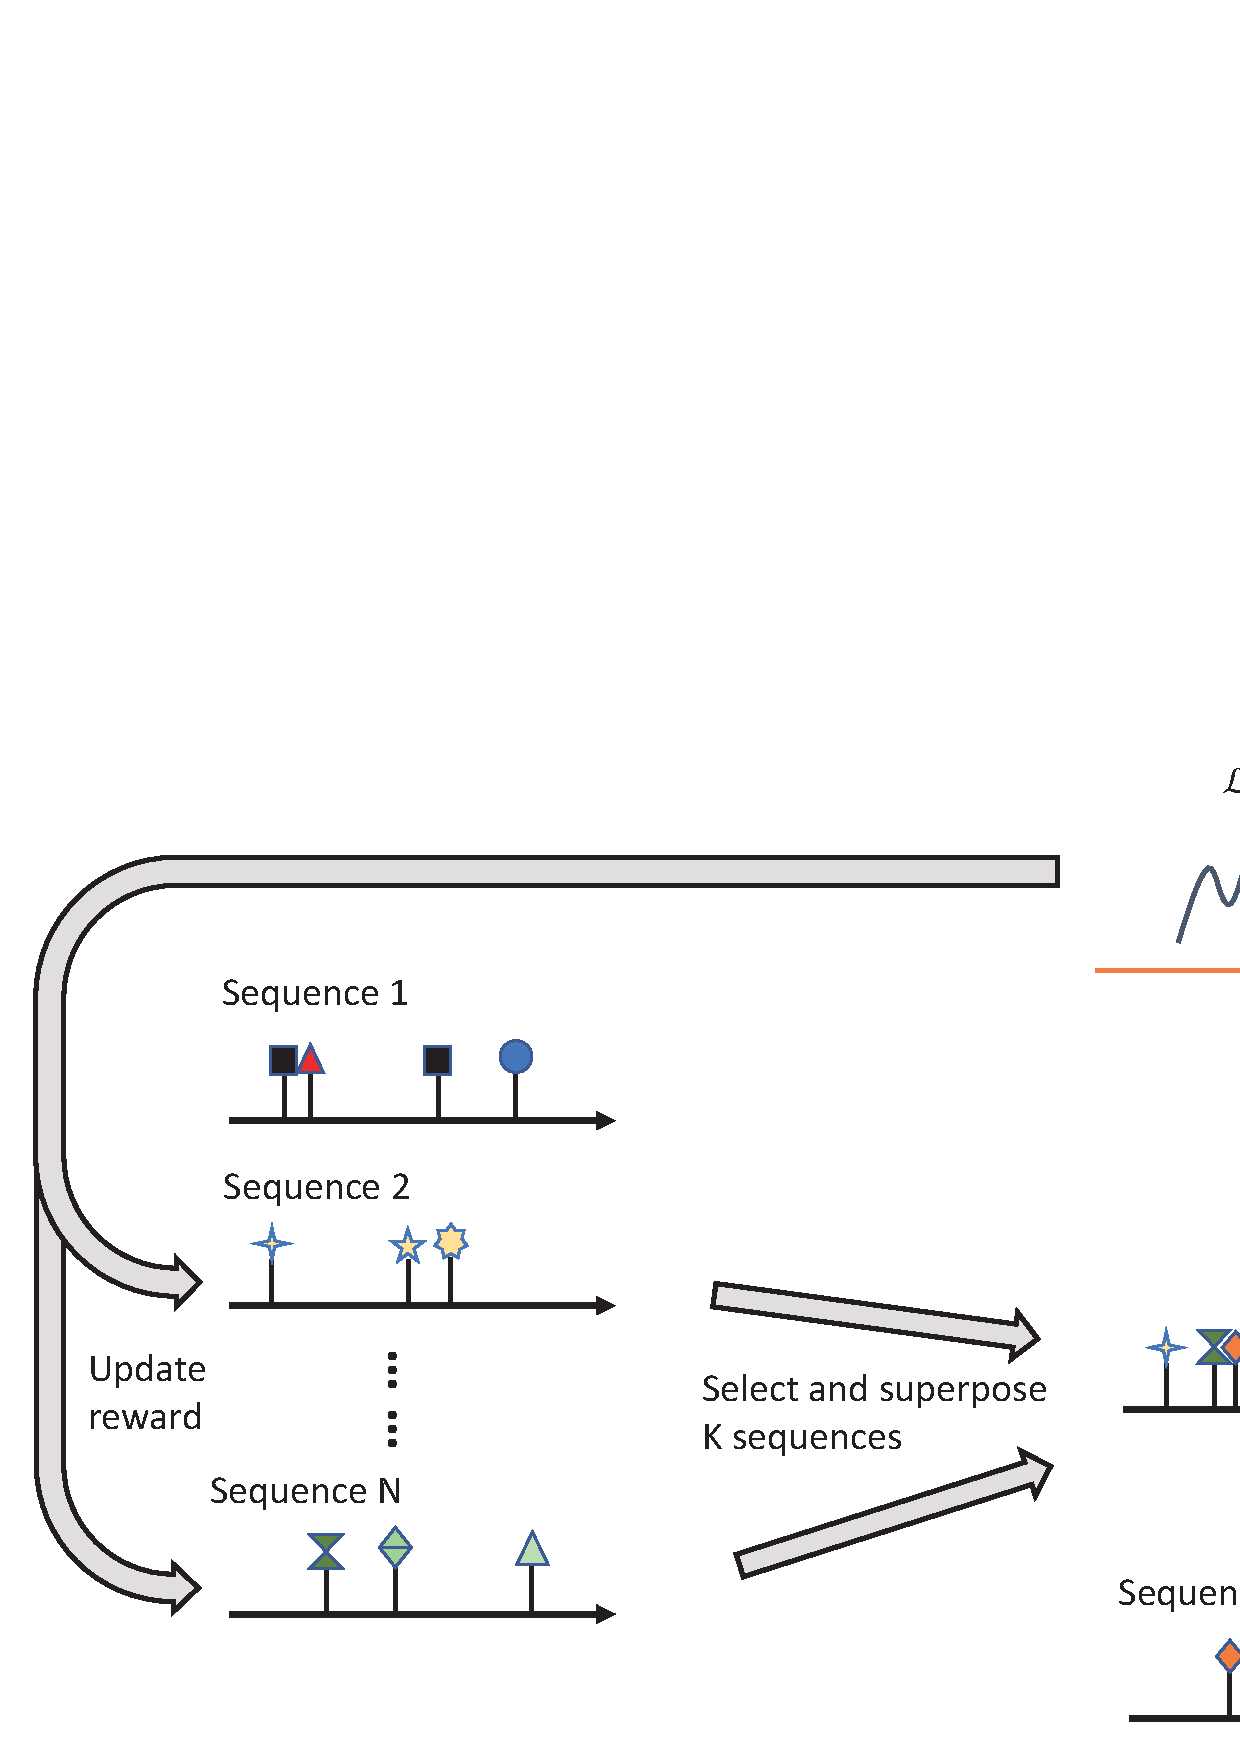
\includegraphics[height=6cm]{figure1.jpg}
\end{figure}
\end{frame}


% The second approach to model network formation is agent- or game theory-based modelling. In these models, a network with fixed number of nodes or agents is created. Every agent is given utility function, a representation of its linking preferences, and directed to form links with other nodes based upon it. Usually, forming or maintaining a link will have a cost, but having connections to other nodes will have benefits. The method tests the hypothesis that, given some initial setting and parameter values, a certain network structure will emerge as an equilibrium of this game. Since the number of nodes usually fixed, they can very rarely explain the properties of huge real-world networks; however, they are very useful to examine the network formation in smaller groups.



\begin{frame}{Introduction}

This author derives a tractable approximation to the distribution of network links using many-player asymptotics. And he demonstrates convergence of the link frequency distribution from finite pairwise stable networks to the (many-player) limiting distribution. 


\end{frame}






\begin{frame}[noframenumbering]

\begin{itemize}

    \begin{LARGE}
    
    \item \light{Introduction}
    
    \item Model Description
    
    \item \light{Asymptotic Representation of Network}
    
    \item \light{Convergence to the Limiting Distribution}

    \end{LARGE}
    
\end{itemize}
	
\end{frame}








\begin{frame}{Model Description}

\begin{itemize}
    \item $\mathcal{N}=\left\{ 1,\ldots,n \right\}$ is the set of n agents or nodes.
    \pause
    \item Each agent is associated with a vector of exogenous attributes (types) $x_i \in \mathcal{X}$.
    \pause
    \item $\bm{L}$ is the adjacency matrix, where the element
        \begin{align}
            L_{ij} = 
                \begin{cases}
                1\ & if\ there\ is\ a\ direct\ link\ from\ node\ i\ to\ node\ j\\
                ~\\
                0\ & otherwise
                \end{cases}
        \end{align}
    \pause
    \item Player i’s payoffs are of the form 
        \begin{align}
            \Pi_i(\bm{L}) = B_i(\bm{L}) - C_i(\bm{L})
        \end{align}
        
    
\end{itemize}


    
\end{frame}



















\begin{frame}{Model Description}

\begin{itemize}
    \item the incremental benefit of adding a link ij
    \begin{align}
        U_{ij}(\bm{L}) := B_i(\bm{L} + \left\{ ij \right\}) - B_i(\bm{L} - \left\{ ij \right\})
    \end{align}
    
    \item the cost increment of adding that link
    \begin{align}
        MC_{ij}(\bm{L}) := C_i(\bm{L} + \left\{ ij \right\}) - C_i(\bm{L} - \left\{ ij \right\})
    \end{align}
    \pause
    
    \item this paper specifies the marginal benefit function as
    \begin{align}
        U_{ij}(\bm{L}) = U_{ij}^*(\bm{L}) + \sigma \eta_{ij}
    \end{align}
    
    \item and marginal costs as
    \begin{align}
        MC_{ij}(\bm{L}) := \max_{k=1,\ldots,J} \sigma \eta_{i0,k}
    \end{align}
        
    
\end{itemize}


    
\end{frame}








\begin{frame}{Model Description}

\begin{itemize}
    \item Node-specific network statistics
    \begin{align}
        S_1(\bm{L}, \bm{X};i) := \sum_{j \ne i} L_{ij}
    \end{align}
    
    \item 
    \begin{align}
        S_2(\bm{L}, \bm{X};i) := \frac{\sum_{j \ne i} L_{ij} \bm{1} \left\{ x_{jk} = \bar{x}_k \right\}}{\sum_{j \ne i} L_{ij}}
    \end{align}
    \pause
    
    \item Edge-specific network statistics
    \begin{align}
        T_1(\bm{L}, \bm{X};i,j) = \sum_{k \ne i,j} L_{ik} L_{jk}
    \end{align}
    
    \item 
    \begin{align}
        T_2(\bm{L}, \bm{X};i,j) = \max \left\{ L_{ik} L_{jk} : k \ne i,j \right\}
    \end{align}
        
    
\end{itemize}


    
\end{frame}










\begin{frame}{Model Description}

The marginal benefit function can be defined as

\begin{align}
    U_{ij}^*(\bm{L}) \equiv U^*(x_i, x_j; S_i, S_j, T_{ij})
\end{align}

\end{frame}













\begin{frame}{Pairwise Stable Network}

$\bm{Definition\ 1\ (Pairwise\ Stable\ Network)}$ The undirected graph $\bm{L}$ is a pairwise
stable network (PSN) if for any link ij with $L_{ij}=1$,
\begin{align*}
    \Pi_i(\bm{L}) \ge \Pi_i(\bm{L} - \left\{ ij \right\}), and\ \Pi_j(\bm{L}) \ge \Pi_j(\bm{L} - \left\{ ij \right\})
\end{align*}
and any link ij with $L_{ij}=0$,
\begin{align*}
     \Pi_i(\bm{L} + \left\{ ij \right\}) < \Pi_i(\bm{L}), or\ \Pi_j(\bm{L} + \left\{ ij \right\}) < \Pi_j(\bm{L}) 
\end{align*}



\end{frame}








\begin{frame}[noframenumbering]

\begin{itemize}

    \begin{LARGE}
    
    \item \light{Introduction}
    
    \item \light{Model Description}
    
    \item Asymptotic Representation of Network
    
    \item \light{Convergence to the Limiting Distribution}

    \end{LARGE}
    
\end{itemize}
	
\end{frame}









\begin{frame}{Link Frequency Distribution}

\begin{align}
\begin{split}
    & F_n(x_1, x_2; s_1, s_2, t_{12}):= \\
    & \frac{1}{n} \sum_{i=1}^n \sum_{j \ne i} P(L_{ij}=1, x_i \leq x_1, x_j \leq x_2, s_i \leq s_1 , s_j \leq s_2, t_{ij} \leq t_{12} )
\end{split}
\end{align}




\end{frame}





\begin{frame}{Limiting Model $\mathcal{F}_0^*$}

The limiting model $\mathcal{F}_0^*$ can be described in terms of pairwise stable subnetworks on finite network neighborhoods $\mathcal{N}_{ij}$ around a pair of nodes $i, j$.

~\\
The model $\mathcal{F}_0^*$ describes the distribution generating the network neighborhoods $\mathcal{N}_{ij}$ in the many-player limit as well as the distribution of network outcomes on these neighborhoods.

\end{frame}




\begin{frame}{Limiting Model $\mathcal{F}_0^*$}

The distribution can be described in terms of three components:
\begin{itemize}
    \item the $\bm{reference\ distribution}$  $M^*$ which is a cross-sectional p.d.f. of potential outcomes for the endogenous node characteristics $s_l$ and $t_{l\cdot}$ given exogenous attributes in the relevant subnetwork.
    \item the $\bm{inclusive\ value\ function}$ $H^*(x,s)$ which gives a sufficient statistic for the link opportunity set $W_i(\bm{L}^*)$ of a node with characteristics $x_i=x$ and $s_i=s$ with respect to her link formation decisions.
    \item the $\bm{edge-level\ response}$ $Q^*(l_{12},s_1,s_2,t_{12}|x_1,x_2):=Q^*(l_{12},s_1,s_2,t_{12}|x_1,x_2;H^*,M^*)$ which corresponds to a conditional probability of a link $ij$ forming together with the resulting values of the endogenous network variables $s_1, s_2, t_{12}$.
\end{itemize}



\end{frame}









\begin{frame}{Limiting Model $\mathcal{F}_0^*$}

The resulting limiting link frequency distribution has p.d.f.
\begin{align}
\begin{split}
    f_0^*(x_1, x_2;s_1, s_2) = 
    & \frac{s_{11} s_{12} \exp \left\{ U^*(x_1, x_2; s_1, s_2) + U^*(x_2, x_1;s_2, s_1)\right\}}{(1+H^*(x_1, s_1))(1+H^*(x_2,s_2))} \\
    & \times M^*(s_1|x_1, x_2) M^*(s_2|x_2, x_1) w(x_1) w(x_2)
\end{split}
\end{align}


\end{frame}







\begin{frame}{Limiting Model $\mathcal{F}_0^*$}

The inclusive value function $H^*(x_1,s_1)$ is a nonnegative function satisfying the fixed-point condition
\begin{align}
    H^*(x;s) = \Psi_0[H^*, M^*](x;s)
\end{align}
where the fixed-point operator $\Psi_0$
\begin{align}
\begin{split}
     \Psi_0[H,M](x;s):=\int & \frac{s_{12} \exp \left\{ U^*(x,x_2;s,s_2) + U^*(x_2,x;s_2,s)\right\}}{1+H(x_2;s_2)} \\
     & \times M^*(s_2|x_2,x_1) w(x_2) ds_2 dx_2
\end{split}
\end{align}

\end{frame}







\begin{frame}{Limiting Model $\mathcal{F}_0^*$}

The reference distribution
\begin{align}
    M^*(s_1|x_1, x_2) = \Omega_0[H^*, M^*](x_1, x_2;s_1)
\end{align}
where the operator $\Omega_0$ maps $H, M$ to the conditional distribution for the network statistic $s_i$ given $x_i$ resulting from the edge-level response in the cross section.

~\\
In the case of no endogenous interaction effects, 
\begin{align}
    \Omega_0[H,M](x_1, x_2;s_{11}) := \frac{H(x_1)^{s_{11}}}{(1+H^*(x_1))^{s_{11}+1}}
\end{align}

\end{frame}





\begin{frame}[noframenumbering]

\begin{itemize}

    \begin{LARGE}
    
    \item \light{Introduction}
    
    \item \light{Model Description}
    
    \item \light{Asymptotic Representation of Network}
    
    \item Convergence to the Limiting Distribution

    \end{LARGE}
    
\end{itemize}
	
\end{frame}











\begin{frame}{Convergence to the Limiting Distribution}



$\bm{Assumption\ 1\ (Systematic\ Part\ of\ Payoffs)}$(i) The systematic parts of payoffs are uniformly bounded in absolute value for some value of $t=t_0, |U^*(x,x',s,s',t_0)| \leq \bar{U} < \infty $. Furthermore, (ii) at all values of $s, s'$, the function $U^*(x,x',s,s',t_0)$ is $p \ge 1$ times differentiable in $x$ with uniformly bounded partial derivatives. (iii) The supports of the payoff-relevant network statistics, $\mathcal{S}$ and $\mathcal{T}$ , and the type space $\mathcal{X}$ are compact sets.




\end{frame}








\begin{frame}{Convergence to the Limiting Distribution}

$\bm{Assumption\ 2\ (Idiosyncratic\ Part\ of\ Payoffs)}$ $\eta_{ij}$ and $\eta_{i0,k}$ are i.i.d. draws from the distribution $G(s)$, and are independent of $x_i, x_j$, where (i) the c.d.f. $G(s)$ is absolutely continuous with density $g(s)$, and (ii) the upper tail of the distribution $G(s)$ is of type I with
auxiliary function $a(s):= \frac{1-G(s)}{g(s)}$ .




\end{frame}







\begin{frame}{Convergence to the Limiting Distribution}

$\bm{Assumption\ 3\ (Network\ Size)}$(i) The number $n$ of agents in the network grows to infinity, and (ii) the random draws for marginal costs $MC_i$ are governed by the sequence $J=[n^{1/2}]$, where $[x]$ denotes the value of $x$ rounded to the closest integer. (iii) The scale parameter for the taste shifters $\sigma \equiv \sigma_n = \frac{1}{a(b_n)}$, where $b_n = G^{-1} (1-\frac{1}{\sqrt{n}})$, and $a(s)$ is the auxiliary function specified in Assumption 2 (ii). Furthermore, (iv) for any values $t_1 \ne t_2 \in \mathcal{T}, |U(x,x',s,s',t_1)-U(x,x',s,s',t_2)|$ may increase with $n$, and there exists a constant $B_T < \infty$ such that for any sequence of pairwise stable networks $(\bm{L}_n^*)_{n \ge 2}$, $\sup_{x,x',s,s'} \left( \mathbb{E}[\exp \left\{ 2|U(x,x',s,s',T(\bm{L}_n^*,x,x',i,j)) - U(x,x',s,s',t_0)| \right\}] \right)^(1/2) \leq \exp \left\{ B_T \right\}$ for $n$ sufficiently large.




\end{frame}







\begin{frame}{Convergence to the Limiting Distribution}

$\bm{Assumption\ 4\ (Pairwise\ Stability)}$ Let $\mathcal{N}_s \subset \left\{ 1,\ldots, n  \right\}$ be the subset of nodes for which the network $L^*$ satisfies the payoff conditions for pairwise stability in Definition 1. Then for any $\epsilon > 0, |\mathcal{N}_s|/n > 1 - \epsilon$ with probability approaching 1 as $n$ increases.




\end{frame}








\begin{frame}{Convergence to the Limiting Distribution}

$\bm{Assumption\ 5\ }$  (i) The mapping $\Omega_0$ is compact and upper hemi-continuous in $H,\ M$ for all $x \in \mathcal{X} $ and $S \subset \mathcal{R}$, and (ii) the core of $\Omega_0[H,M]$ is nonempty, where the boundary of the core of $\Omega_0[H,M]$ is in some compact subset $\mathcal{U} \subset \Delta (\mathcal{X} \times \mathcal{R})$ for all values of $H,\ M$. (iii)
$\sup_{x, Z \subset \mathcal{R}} |\hat{\Omega}_n[H,M](Z) - \Omega_0[H,M](Z)| \to 0$ uniformly in $H \in \mathcal{G}$ and distributions $M \in \mathcal{U}$.




\end{frame}




\begin{frame}{Convergence to the Limiting Distribution}

$\bm{Theorem\  1\ (Fixed\ Point\ Existence)}$Suppose that Assumptions 1 and 5 (i)-(ii) hold. Then the mapping $(H,M) \to (\Psi_0,\Omega_0)$ has a fixed point.

~\\
$\bm{Theorem\ 2\ (Convergence)}$ Suppose that Assumptions 1-5 hold, and let $\mathcal{F}_0^*$ be the set of distributions characterized by (13) (14) and (16). Then for any pairwise or cyclically stable network there exists a distribution $F_0^*(x_1, x_2; s_1, s_2) \in \mathcal{F}_0^*$ such that the link frequency distribution
\begin{align*}
    \sup_{x_1,x_2,s_1,s_2,t_{12}} |\hat{F}_n(x_1,x_2;s_1,s_2,t_{12}) - F_0^*(x_1,x_2;s_1,s_2,t_{12})| = o_p(1)
\end{align*}
Furthermore, convergence is uniform with respect to selection among pairwise stable networks.

\end{frame}




\end{document}	% Done!

